% Created 2025-06-30 Mon 15:34
% Intended LaTeX compiler: pdflatex
\documentclass[bigger,aspectratio=169]{beamer}
  \usepackage{caption, subcaption, csquotes, amssymb, xcolor}
\usepackage[english]{babel}
\titlegraphic{\includesvg[height=1cm]{./figs/IE_Unicamp}\hspace*{1.25cm}\includesvg[height=1cm]{./figs/SSSA}\hspace*{1.25cm} \includesvg[height=1cm]{./figs/YSI}}
\AtBeginSection[]{
\begin{frame}{Outline}
\tableofcontents[currentsection]
\end{frame}
}
\usepackage[utf8]{inputenc}
\usepackage[T1]{fontenc}
\usepackage{amsmath}
\usepackage{amsfonts}
\usepackage{amssymb}
\usepackage{multicol}
\usepackage{graphicx}
\usepackage{textpos}
\usepackage{caption}
\usepackage{subfig}
\usepackage{svg}
\usepackage{pgfpages}
\usepackage{epstopdf}
\epstopdfsetup{update} % only regenerate if changed
\DeclareGraphicsRule{.eps}{pdf}{.pdf}{`epstopdf #1}
\usepackage{tikz}
\usetikzlibrary{arrows.meta, positioning, shapes}
\usepackage{fontawesome5}
\usetheme{metropolis}
\usecolortheme{beaver}
\author{Gabriel Petrini}
\date{July, 2025}
\title{ABM Macro Lab: Agent-based Modelling Tools}
\subtitle{Session 02}
\hypersetup{
 pdfauthor={Gabriel Petrini},
 pdftitle={ABM Macro Lab: Agent-based Modelling Tools},
 pdfkeywords={},
 pdfsubject={},
 pdfcreator={Emacs 29.3 (Org mode 9.7.31)}, 
 pdflang={English}}

% Setup for code blocks [1/2]

\usepackage{fvextra}

\fvset{%
  commandchars=\\\{\},
  highlightcolor=white!95!black!80!blue,
  breaklines=true,
  breaksymbol=\color{white!60!black}\tiny\ensuremath{\hookrightarrow}}

% Make line numbers smaller and grey.
\renewcommand\theFancyVerbLine{\footnotesize\color{black!40!white}\arabic{FancyVerbLine}}

\usepackage{xcolor}

% In case engrave-faces-latex-gen-preamble has not been run.
\providecolor{EfD}{HTML}{f7f7f7}
\providecolor{EFD}{HTML}{28292e}

% Define a Code environment to prettily wrap the fontified code.
\usepackage[breakable,xparse]{tcolorbox}
\DeclareTColorBox[]{Code}{o}%
{colback=EfD!98!EFD, colframe=EfD!95!EFD,
  fontupper=\footnotesize\setlength{\fboxsep}{0pt},
  colupper=EFD,
  IfNoValueTF={#1}%
  {boxsep=2pt, arc=2.5pt, outer arc=2.5pt,
    boxrule=0.5pt, left=2pt}%
  {boxsep=2.5pt, arc=0pt, outer arc=0pt,
    boxrule=0pt, leftrule=1.5pt, left=0.5pt},
  right=2pt, top=1pt, bottom=0.5pt,
  breakable}

% Support listings with captions
\usepackage{float}
\floatstyle{plain}
\newfloat{listing}{htbp}{lst}
\newcommand{\listingsname}{Listing}
\floatname{listing}{\listingsname}
\newcommand{\listoflistingsname}{List of Listings}
\providecommand{\listoflistings}{\listof{listing}{\listoflistingsname}}


% Setup for code blocks [2/2]: syntax highlighting colors

\newcommand\efstrut{\vrule height 2.1ex depth 0.8ex width 0pt}
\definecolor{EFD}{HTML}{383a42}
\definecolor{EfD}{HTML}{fafafa}
\newcommand{\EFD}[1]{\textcolor{EFD}{#1}} % default
\newcommand{\EFvp}[1]{#1} % variable-pitch
\definecolor{EFh}{HTML}{9ca0a4}
\newcommand{\EFh}[1]{\textcolor{EFh}{#1}} % shadow
\definecolor{EFsc}{HTML}{50a14f}
\newcommand{\EFsc}[1]{\textcolor{EFsc}{#1}} % success
\definecolor{EFw}{HTML}{986801}
\newcommand{\EFw}[1]{\textcolor{EFw}{#1}} % warning
\definecolor{EFe}{HTML}{e45649}
\newcommand{\EFe}[1]{\textcolor{EFe}{#1}} % error
\definecolor{Efl}{HTML}{c6c7c7}
\newcommand{\EFl}[1]{\colorbox{Efl}{\efstrut{}\textbf{#1}}} % link
\definecolor{EFlv}{HTML}{8b008b}
\definecolor{Eflv}{HTML}{c6c7c7}
\newcommand{\EFlv}[1]{\colorbox{Eflv}{\efstrut{}\textcolor{EFlv}{\textbf{#1}}}} % link-visited
\definecolor{EFhi}{HTML}{f0f0f0}
\definecolor{Efhi}{HTML}{4078f2}
\newcommand{\EFhi}[1]{\colorbox{Efhi}{\efstrut{}\textcolor{EFhi}{#1}}} % highlight
\definecolor{EFc}{HTML}{9ca0a4}
\newcommand{\EFc}[1]{\textcolor{EFc}{#1}} % font-lock-comment-face
\definecolor{EFcd}{HTML}{9ca0a4}
\newcommand{\EFcd}[1]{\textcolor{EFcd}{#1}} % font-lock-comment-delimiter-face
\definecolor{EFs}{HTML}{50a14f}
\newcommand{\EFs}[1]{\textcolor{EFs}{#1}} % font-lock-string-face
\definecolor{EFd}{HTML}{84888b}
\newcommand{\EFd}[1]{\textcolor{EFd}{\textit{#1}}} % font-lock-doc-face
\definecolor{EFm}{HTML}{b751b6}
\newcommand{\EFm}[1]{\textcolor{EFm}{#1}} % font-lock-doc-markup-face
\definecolor{EFk}{HTML}{e45649}
\newcommand{\EFk}[1]{\textcolor{EFk}{#1}} % font-lock-keyword-face
\definecolor{EFb}{HTML}{a626a4}
\newcommand{\EFb}[1]{\textcolor{EFb}{#1}} % font-lock-builtin-face
\definecolor{EFf}{HTML}{a626a4}
\newcommand{\EFf}[1]{\textcolor{EFf}{#1}} % font-lock-function-name-face
\definecolor{EFv}{HTML}{6a1868}
\newcommand{\EFv}[1]{\textcolor{EFv}{#1}} % font-lock-variable-name-face
\definecolor{EFt}{HTML}{986801}
\newcommand{\EFt}[1]{\textcolor{EFt}{#1}} % font-lock-type-face
\definecolor{EFo}{HTML}{b751b6}
\newcommand{\EFo}[1]{\textcolor{EFo}{#1}} % font-lock-constant-face
\definecolor{EFwr}{HTML}{986801}
\newcommand{\EFwr}[1]{\textcolor{EFwr}{#1}} % font-lock-warning-face
\definecolor{EFnc}{HTML}{4078f2}
\newcommand{\EFnc}[1]{\textcolor{EFnc}{\textbf{#1}}} % font-lock-negation-char-face
\definecolor{EFpp}{HTML}{4078f2}
\newcommand{\EFpp}[1]{\textcolor{EFpp}{\textbf{#1}}} % font-lock-preprocessor-face
\definecolor{EFrc}{HTML}{4078f2}
\newcommand{\EFrc}[1]{\textcolor{EFrc}{\textbf{#1}}} % font-lock-regexp-grouping-construct
\definecolor{EFrb}{HTML}{4078f2}
\newcommand{\EFrb}[1]{\textcolor{EFrb}{\textbf{#1}}} % font-lock-regexp-grouping-backslash
\definecolor{Efob}{HTML}{e7e7e7}
\newcommand{\EFob}[1]{\colorbox{Efob}{\efstrut{}#1}} % org-block
\definecolor{Efobb}{HTML}{e7e7e7}
\newcommand{\EFobb}[1]{\colorbox{Efobb}{\efstrut{}\textit{#1}}} % org-block-begin-line
\definecolor{Efobe}{HTML}{e7e7e7}
\newcommand{\EFobe}[1]{\colorbox{Efobe}{\efstrut{}\textit{#1}}} % org-block-end-line
\definecolor{EFOa}{HTML}{e45649}
\newcommand{\EFOa}[1]{\textcolor{EFOa}{\textbf{#1}}} % outline-1
\definecolor{EFOb}{HTML}{da8548}
\newcommand{\EFOb}[1]{\textcolor{EFOb}{\textbf{#1}}} % outline-2
\definecolor{EFOc}{HTML}{b751b6}
\newcommand{\EFOc}[1]{\textcolor{EFOc}{\textbf{#1}}} % outline-3
\definecolor{EFOd}{HTML}{6f99f5}
\newcommand{\EFOd}[1]{\textcolor{EFOd}{\textbf{#1}}} % outline-4
\definecolor{EFOe}{HTML}{bc5cba}
\newcommand{\EFOe}[1]{\textcolor{EFOe}{\textbf{#1}}} % outline-5
\definecolor{EFOf}{HTML}{9fbbf8}
\newcommand{\EFOf}[1]{\textcolor{EFOf}{\textbf{#1}}} % outline-6
\definecolor{EFOg}{HTML}{d292d1}
\newcommand{\EFOg}[1]{\textcolor{EFOg}{\textbf{#1}}} % outline-7
\definecolor{EFOh}{HTML}{d8e4fc}
\newcommand{\EFOh}[1]{\textcolor{EFOh}{\textbf{#1}}} % outline-8
\newcommand{\EFhn}[1]{#1} % highlight-numbers-number
\newcommand{\EFhq}[1]{#1} % highlight-quoted-quote
\newcommand{\EFhs}[1]{#1} % highlight-quoted-symbol
\newcommand{\EFrda}[1]{#1} % rainbow-delimiters-depth-1-face
\newcommand{\EFrdb}[1]{#1} % rainbow-delimiters-depth-2-face
\newcommand{\EFrdc}[1]{#1} % rainbow-delimiters-depth-3-face
\newcommand{\EFrdd}[1]{#1} % rainbow-delimiters-depth-4-face
\newcommand{\EFrde}[1]{#1} % rainbow-delimiters-depth-5-face
\newcommand{\EFrdf}[1]{#1} % rainbow-delimiters-depth-6-face
\newcommand{\EFrdg}[1]{#1} % rainbow-delimiters-depth-7-face
\newcommand{\EFrdh}[1]{#1} % rainbow-delimiters-depth-8-face
\newcommand{\EFrdi}[1]{#1} % rainbow-delimiters-depth-9-face
\definecolor{EFany}{HTML}{986801}
\definecolor{Efany}{HTML}{986801}
\newcommand{\EFany}[1]{\colorbox{Efany}{\efstrut{}\textcolor{EFany}{#1}}} % ansi-color-yellow
\definecolor{EFanr}{HTML}{e45649}
\definecolor{Efanr}{HTML}{e45649}
\newcommand{\EFanr}[1]{\colorbox{Efanr}{\efstrut{}\textcolor{EFanr}{#1}}} % ansi-color-red
\definecolor{EFanb}{HTML}{fafafa}
\newcommand{\EFanb}[1]{\textcolor{EFanb}{#1}} % ansi-color-black
\definecolor{EFang}{HTML}{50a14f}
\definecolor{Efang}{HTML}{50a14f}
\newcommand{\EFang}[1]{\colorbox{Efang}{\efstrut{}\textcolor{EFang}{#1}}} % ansi-color-green
\definecolor{EFanB}{HTML}{4078f2}
\definecolor{EfanB}{HTML}{4078f2}
\newcommand{\EFanB}[1]{\colorbox{EfanB}{\efstrut{}\textcolor{EFanB}{#1}}} % ansi-color-blue
\definecolor{EFanc}{HTML}{0184bc}
\definecolor{Efanc}{HTML}{0184bc}
\newcommand{\EFanc}[1]{\colorbox{Efanc}{\efstrut{}\textcolor{EFanc}{#1}}} % ansi-color-cyan
\definecolor{Efanw}{HTML}{383a42}
\newcommand{\EFanw}[1]{\colorbox{Efanw}{\efstrut{}#1}} % ansi-color-white
\definecolor{EFanm}{HTML}{a626a4}
\definecolor{Efanm}{HTML}{a626a4}
\newcommand{\EFanm}[1]{\colorbox{Efanm}{\efstrut{}\textcolor{EFanm}{#1}}} % ansi-color-magenta
\definecolor{EFANy}{HTML}{a77e27}
\definecolor{EfANy}{HTML}{a77e27}
\newcommand{\EFANy}[1]{\colorbox{EfANy}{\efstrut{}\textcolor{EFANy}{#1}}} % ansi-color-bright-yellow
\definecolor{EFANr}{HTML}{e86f64}
\definecolor{EfANr}{HTML}{e86f64}
\newcommand{\EFANr}[1]{\colorbox{EfANr}{\efstrut{}\textcolor{EFANr}{#1}}} % ansi-color-bright-red
\definecolor{EFANb}{HTML}{9ca0a4}
\definecolor{EfANb}{HTML}{9ca0a4}
\newcommand{\EFANb}[1]{\colorbox{EfANb}{\efstrut{}\textcolor{EFANb}{#1}}} % ansi-color-bright-black
\definecolor{EFANg}{HTML}{6aaf69}
\definecolor{EfANg}{HTML}{6aaf69}
\newcommand{\EFANg}[1]{\colorbox{EfANg}{\efstrut{}\textcolor{EFANg}{#1}}} % ansi-color-bright-green
\definecolor{EFANB}{HTML}{5c8cf3}
\definecolor{EfANB}{HTML}{5c8cf3}
\newcommand{\EFANB}[1]{\colorbox{EfANB}{\efstrut{}\textcolor{EFANB}{#1}}} % ansi-color-bright-blue
\definecolor{EFANc}{HTML}{2796c6}
\definecolor{EfANc}{HTML}{2796c6}
\newcommand{\EFANc}[1]{\colorbox{EfANc}{\efstrut{}\textcolor{EFANc}{#1}}} % ansi-color-bright-cyan
\definecolor{EFANw}{HTML}{1b2229}
\definecolor{EfANw}{HTML}{1b2229}
\newcommand{\EFANw}[1]{\colorbox{EfANw}{\efstrut{}\textcolor{EFANw}{#1}}} % ansi-color-bright-white
\definecolor{EFANm}{HTML}{b346b1}
\definecolor{EfANm}{HTML}{b346b1}
\newcommand{\EFANm}[1]{\colorbox{EfANm}{\efstrut{}\textcolor{EFANm}{#1}}} % ansi-color-bright-magenta
\usepackage[style=authoryear]{biblatex}
\addbibresource{~/Org/zotero_refs.bib}
\begin{document}

\maketitle
\begin{frame}{Outline}
\tableofcontents
\end{frame}

\section{Technical review}
\label{sec:org8389284}

\begin{frame}[label={sec:orgc375df6}]{Simulation pipeline}
As a recap, whenever running a model on LSD, we need to:

\begin{enumerate}
\item Design a model (on paper);
\item Write the code implementing the equation;
\item Define the model structure and initialization;
\item Run the simulation;
\item Analyze the results.
\end{enumerate}
\begin{block}{Where are we and where are we going?}
In the previous session, we implemented two different small models.
Now, we will focus on a economic ABM.
\end{block}
\end{frame}
\section{Theoretical model presentation}
\label{sec:orgfdd8103}


\begin{frame}[label={sec:org976ee91},fragile]{Sequence of events}
 At time \(t = 0\), there are \(NF\) identical incumbent firms with equal \(a_{i,t=0}\) and \(s_{i,0}\).
At each time step \(t = 1, 2, \ldots, T\):
\begin{enumerate}
\item Firms learn (updates (\(a_{i}\)))
\item Firms computes market share (updates \(s_{i}\))
\item Market concentration index (\(HHI\)) is computed
\item Firms exits the market if \(s_{i} < s_{min}\)
\item Firms enter to keep \(NF\) firms in the market
\item Incumbents variables (\(a_{j}\), \(s_{j}\)) are set
\item Market shares are re-scaled proportionally to ensure \(\sum s_{i} = 1\)
\end{enumerate}
\begin{block}{Model logical order (later)}
The exit-entry process is time-coordinated during each simulated time step by the technical variable \texttt{exit\_entry}: \texttt{HHI} > \texttt{exit\_decision} > \texttt{s} rescaling
\end{block}
\end{frame}
\begin{frame}[label={sec:orgb384df1}]{Equations}
\[ \begin{array}{lrl}
\mbox{Idiosyncratic learning process:} & a_{i,t} = &a_{i,t-1}\cdot (1 + \eta\cdot\theta_{i,t})\\
\mbox{Learning shocks} & \theta_{i,t} \sim  & Beta(\beta_1, \beta_2)\\
\mbox{Market selection} & s_{i,t} =  & s_{i,t-1} \cdot \left( 1 + A\cdot\frac{a_{i,t} - \bar{a}_{t}}{\bar{a}_{t}}\right) \\
\mbox{Average productivity} & \bar{a}_{t} =  & \sum_{i=1}^{NF} s_{i, t-1}\cdot a_{i,t} \\
\mbox{Exit condition} & s_{i,t} < & s_{min}\\
\mbox{Entrant productivity} & a_{j,t} =&  \bar{a}_{t}\cdot (1 + \eta\cdot\theta_{i,t})\\
\mbox{Entrant market-share} & s_{j,t} =& 1/NF \\
\mbox{Market concentration index} & HHI_{t} =& \sum_{i=1}^{NF} (s_{i})^2 \\
\mbox{Market-share adjustment} &  s_{i} \mapsto & s_{i}\cdot \frac{1}{\sum_{i=1}^{NF} s_{i}} \Rightarrow \sum_{i=1}^{NF} s_{i} = 1 \\
\mbox{Fixed number of firms} & \#\{1, \ldots, n\} =& NF
\end{array}\]
\end{frame}
\begin{frame}[label={sec:org23d29c7}]{Parameters and initial values}
\begin{table}[htbp]
\caption{Baseline parameters}
\centering
\begin{tabular}{ccc}
\hline
 & Desc & Value\\
\hline
\(\eta\) & Innovation opportunity support & 0.3\\
\(\beta_{1}, \beta_{2}\) & beta distribution parameters & 1.0; 5.0\\
\(A\) & replicator dynamics intensity & 1\\
\(s_{min}\) & minimum market share to not exit & 0.01\\
\(NF\) & number of firms & 10\\
\hline
\(a_{i}_{}\) & Initial Firm-level productivity & 1.0\\
\(s_{i}\) & Initial Firm market-share & \(1/NF\)\\
\hline
\end{tabular}
\end{table}
\end{frame}
\begin{frame}[label={sec:org18450f1}]{Model structure and data organization}
\begin{figure}[htbp]
\centering
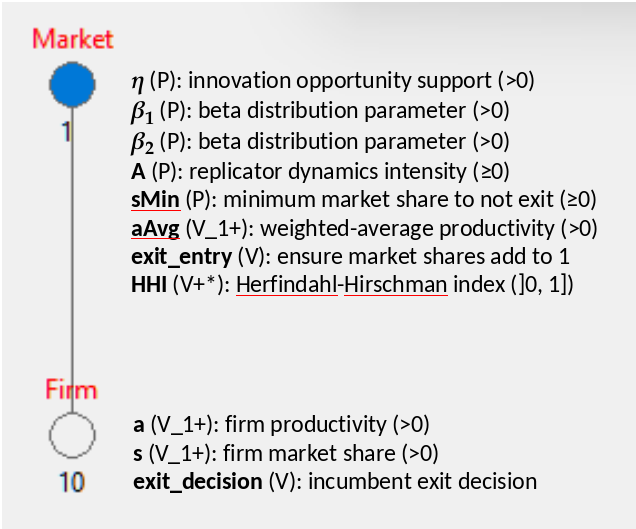
\includegraphics[clip,trim=0 0 0 0,width=.8\textwidth,height=.75\textheight]{figs/Structure_Industry_LSD.png}
\caption{Structure of industry model}
\end{figure}
\end{frame}
\section{Model implementation}
\label{sec:orge4a5b55}

\begin{frame}[label={sec:orgda6f275},fragile]{Firm-level productivity (\(a_i\))}
 \begin{equation}
a_{i,t} = a_{i,t-1}\cdot (1 + \eta\cdot\theta_{i,t})
\end{equation}


\begin{Code}
\begin{Verbatim}
\color{EFD}\EFo{EQUATION}(\EFs{"a"})
\EFcd{//} \EFc{Firm knowledge/productivity}
v[0] = \EFo{CURRENT};
v[1] = V(\EFs{"eta"}); v[2] = V(\EFs{"beta1"}); v[3] = V(\EFs{"beta2"});
v[4] = beta(v[2], v[3]);
v[5] = v[0] * (1 + v[1] * v[4]);
\EFo{RESULT}(v[5])
\end{Verbatim}
\end{Code}
\begin{block}{One-liner}
\begin{Code}
\begin{Verbatim}
\color{EFD}\EFo{EQUATION}(\EFs{"a"})
\EFo{RESULT}(VL(\EFs{"a"}, 1) * (1 + V(\EFs{"eta"}) * (beta(V(\EFs{"beta1"}), V(\EFs{"beta2"})))))
\end{Verbatim}
\end{Code}
\end{block}
\end{frame}
\begin{frame}[label={sec:org515cd8c},fragile]{Market-share (\(s_{i}\))}
 \begin{equation}
s_{i,t} = s_{i,t-1} \cdot \left( 1 + A\cdot\frac{a_{i,t} - \bar{a}_{t}}{\bar{a}_{t}}\right)
\end{equation}


\begin{Code}
\begin{Verbatim}
\color{EFD}\EFo{EQUATION}(\EFs{"s"})
\EFcd{//} \EFc{Firm size/market share}
v[0] = \EFo{CURRENT};
v[1] = V(\EFs{"A"}); v[2] = V(\EFs{"a"}); v[3] = V(\EFs{"aAvg"});
v[4] = (v[2] - v[3])/v[3];
v[5] = v[0] * (1 + v[1] * v[4]);
\EFo{RESULT}(v[5])
\end{Verbatim}
\end{Code}
\begin{block}{One-liner}
\begin{Code}
\begin{Verbatim}
\color{EFD}\EFo{EQUATION}(\EFs{"s"}) \EFcd{//} \EFc{Firm size/market share}
\EFo{RESULT}(VL(\EFs{"s"}, 1) * (1 + V(\EFs{"A"}) * ((V(\EFs{"a"}) - V(\EFs{"aAvg"}))/V(\EFs{"aAvg"}))))
\end{Verbatim}
\end{Code}
\end{block}
\end{frame}
\begin{frame}[label={sec:org70d3cdd},fragile]{Exit condition}
 \begin{Code}
\begin{Verbatim}
\color{EFD}\EFo{EQUATION}(\EFs{"exit\_decision"})

v[0] = V(\EFs{"s"}); v[1] = V(\EFs{"sMin"});
\EFcd{//} \EFc{update entrant firm productivity and market share}
\EFk{if} (v[0] < v[1]) \{
  v[2] = V(\EFs{"eta"}); v[3] = V(\EFs{"beta1"}); v[4] = V(\EFs{"beta2"});
  v[5] = beta(v[3], v[4]);
  v[6] = V(\EFs{"aAvg"});
  v[7] = v[6] * (1 + v[2] * v[5]);
  \EFo{WRITE}( \EFs{"a"}, v[7] );
  \EFo{WRITE}( \EFs{"s"}, 1 / \EFo{COUNT}( \EFs{"Firm"} ) );
\}
\EFo{RESULT}(0)
\end{Verbatim}
\end{Code}
\end{frame}
\begin{frame}[label={sec:orgd33dd32},fragile]{Market-level Productivity (Weighted) Average (\(\bar{a_{t}}\))}
 \begin{equation}
\bar{a}_{t} =  \sum_{i=1}^{NF} s_{i, t-1}\cdot a_{i,t}
\end{equation}


\begin{Code}
\begin{Verbatim}
\color{EFD}\EFo{EQUATION}( \EFs{"aAvg"} )
\EFcd{//} \EFc{Mean knowledge/productivity}
v[0] = 0;        \EFcd{//} \EFc{accumulator}
\EFv{CYCLE}(cur, \EFs{"Firm"}) \{
  v[1] = \EFo{VLS}( cur, \EFs{"s"}, 1 );
  v[2] = VS( cur, \EFs{"a"} );
  v[3] = v[1] * v[2];
  v[0] += v[3] ;
\}
\EFo{RESULT}( v[0] )
\end{Verbatim}
\end{Code}
\end{frame}
\begin{frame}[label={sec:orga2aa618},fragile]{Entry-Exit condition}
 \begin{Code}
\begin{Verbatim}
\color{EFD}\EFo{EQUATION}( \EFs{"exit\_entry"} )
\EFcd{//} \EFc{Trigger market-wise exit-entry dynamics and re-scale shares}
V( \EFs{"HHI"} ); \EFcd{//} \EFc{first, compute HH index before exits}

\EFcd{//} \EFc{second, ensure firms have decided on exit}
\EFv{CYCLE}(cur, \EFs{"Firm"}) \{VS( cur, \EFs{"exit\_decision"} );\}

v[0] = 1 / \EFo{SUM}( \EFs{"s"} ); \EFcd{//} \EFc{factor to scale back to sum = 1}
\EFv{CYCLE}(cur, \EFs{"Firm"}) \{ \EFcd{//} \EFc{third, rescale market shares after exits}
  v[1] = VS( cur, \EFs{"s"} );
  v[2] = v[0] * v[1];
  \EFo{WRITES}( cur, \EFs{"s"}, v[2]);
\}
\EFo{RESULT}( \EFo{SUM}(\EFs{"s"}) )
\end{Verbatim}
\end{Code}
\end{frame}
\begin{frame}[label={sec:org95f6371},fragile]{Herfindahl-Hirschman concentration index (\(HHI\))}
 \begin{equation}
HHI_{t} = \sum_{i=1}^{NF} (s_{i})^2
\end{equation}


\begin{Code}
\begin{Verbatim}
\color{EFD}\EFo{EQUATION}( \EFs{"HHI"} )
\EFcd{//} \EFc{Herfindahl-Hirschman concentration index}
v[0] = \EFo{WHTAVE}( \EFs{"s"}, \EFs{"s"} );
\EFo{RESULT}( v[0] )
\end{Verbatim}
\end{Code}
\begin{block}{Note on WHTAVE(LS)}
\texttt{WHTAVE} (weighed average, not used here in the strict sense) computes the sum of \(s\times s\) over every firm
\end{block}
\end{frame}
\section{Model initialization}
\label{sec:org1f065e1}

\begin{frame}[label={sec:orgf533b30},fragile]{Initialization I}
 Firm-level initialization can be set for every \(NF\) objects on the LSD browser.
The same applies for every other initial condition.

Whenever changing the number of firms \(NF\), it is important to also a compatible initial market-share \(1/NF\).
This procedure should be done for every firm (instance) of the model.

In the following slide (optional), we will see an alternative way in which we control some few parameters and create \(NF-1\) copies of a example object.

\begin{Code}
\begin{Verbatim}
\color{EFD}\EFo{ADDNOBJ\_EX}(\EFs{"TypeOfAgent"}, number, *pointer);
\end{Verbatim}
\end{Code}
\begin{block}{Semi-automated initialization and sensitivity analysis}
By doing this, we automate the model initialization to test different model configurations (next lecture)
\end{block}
\end{frame}
\begin{frame}[label={sec:org921a147},fragile]{Initialization II}
 \begin{Code}
\begin{Verbatim}
\color{EFD}\EFo{EQUATION}( \EFs{"init"} )
\EFo{PARAMETER};                  \EFcd{//} \EFc{turn into parameter (run once)}
v[0] = V(\EFs{"A0"}); v[1] = V(\EFs{"Nfirm"});
v[2] = 1 / v[1]; \EFcd{//} \EFc{Fair share}
\EFv{CYCLE}(cur, \EFs{"Market"})\{
    cur1 = \EFo{SEARCHS}(cur, \EFs{"Firm"} );
\EFcd{//} \EFc{Overwrites the lag 1 of "a" to v[0] at time 1}
    \EFo{WRITELLS}(cur1, \EFs{"a"}, v[0], 1, 1);
    \EFo{WRITELLS}(cur1, \EFs{"s"}, v[2], 1, 1);
\EFcd{//} \EFc{Adds N - 1 copies of cur1 agent located under cur}
    \EFo{ADDNOBJ\_EXS}(cur, \EFs{"Firm"}, v[1] - 1, cur1);
\}
\EFo{RESULT}( 1 )
\end{Verbatim}
\end{Code}
\end{frame}
\section{Simulations}
\label{sec:org3ffe1fe}

\begin{frame}[label={sec:org0161508}]{Analyzing the model results}
\begin{itemize}
\item After a successful simulation run, in \alert{Browser} click on menu \alert{Data > Analysis of Results}
\item To analyze the \emph{saved} data time series, select the desired variables from the \alert{Series available} list to include them in the \alert{Series selected} list
\item Click on \alert{Plot} button to show the selected variable(s) time series plot
\item Click on \alert{Statistics} button to show the selected time series descriptive statistics in \alert{LSD Log}
\item Plots and analysis data can be \emph{saved} pressing the \alert{Save Plot} and \alert{Save Data} buttons
\end{itemize}
\end{frame}
\begin{frame}[label={sec:orgcb8fa1d}]{Exploring the single run results}
\begin{figure}[ht]
    % First row: Market-level data
    \begin{subfigure}{0.48\textwidth}
        \centering
        \includesvg[width=\linewidth, height=.3\textheight]{./figs/single_avg_log_productivity.svg}
        \caption{Average log-productivity ($a$)}
        \label{fig:avg_prod}
    \end{subfigure}
    \hfill
    \begin{subfigure}{0.48\textwidth}
        \centering
        \includesvg[width=\linewidth, height=.3\textheight]{./figs/single_firm_log_productivity.svg}
        \caption{Firm log-productivity ($a$)}
        \label{fig:firm_prod}
    \end{subfigure}

    % Second row: Firm-level data
    \begin{subfigure}{0.48\textwidth}
        \centering
        \includesvg[width=\linewidth, height=.3\textheight]{./figs/single_HHI.svg}
        \caption{Herfindahl-Hirschman Index (HHI)}
        \label{fig:hhi}
    \end{subfigure}
    \hfill
    \begin{subfigure}{0.48\textwidth}
        \centering
        \includesvg[width=\linewidth, height=.3\textheight]{./figs/single_firm_market_share.svg}
        \caption{Firm market share ($s$)}
        \label{fig:market_share}
    \end{subfigure}
    \label{single-run-industry}
\end{figure}
\end{frame}
\end{document}
